\documentclass[12pt]{article}

\usepackage{listings}
\lstset{
	language=Haskell
}

\usepackage{graphicx}
\graphicspath{ {../../resources/} }

\usepackage[margin=1in]{geometry}

\usepackage{hyperref}

\title{Fibonacci Numbers with Matrices}
\author{Rushi Shah}
\date{9-11-2015}

\begin{document}

	\maketitle
	Ahh, the Fibonacci numbers. What mathemetician doesn't love them?

	Well, in Week 06 of CIS194, some interesting implementations were
	discussed. My favorite (that I never actually had encountered before),
	was in order to get the \texttt{n}'th number, you raise a two by two
	matrix to the \texttt{n}'th power.

	Let's take a look at my implementation:

	\subsection{The Matrix}\label{the-matrix}

	First off, you need to be able to represent matrices. I decided to use a
	tuple of tuples for the two by two matrix.

	\begin{lstlisting}
data Matrix = 	Matrix ((Integer, Integer),
			(Integer, Integer)) 
	\end{lstlisting}

	I also wanted to be able to print them nicely in the terminal, so I
	whipped up a quick show function. I could have derived it, but in my
	opinion, this makes it look slightly nicer (sorry, the function is a bit
	long, so the text wraps).

	\begin{lstlisting}
instance Show Matrix where 
	show (Matrix ((a, b), (c, d))) = 
		"[" ++ show a ++ ", " ++ show b ++ "]"
		"[" ++ show c ++ ", " ++ show d ++ "]"
	\end{lstlisting}

	And now let's instantiate a matrix!

	\begin{lstlisting}
m :: Matrix 
m = Matrix ((1, 1), (1, 0)) 
	\end{lstlisting}

	To check that it works, let's print out the matrix in \texttt{ghci}:

	\begin{lstlisting}
> m
[1, 1]
[1, 0] 
	\end{lstlisting}

	\subsection{Multiplying Matrices}\label{multiplying-matrices}

	So that's great, but these matrices don't really do much. We need to be
	able to raise each matrix to a specific power, but who knows how to do
	that? I sure don't. With that being said, I do know how to multiply two
	2x2 matrices together! Let's define a function \texttt{(*)} that takes
	two 2x2 matrices and returns a matrix representing the multiplication of
	the two arguments. This multiplication function is a part of the
	\texttt{Num} typeclass, so in essence, we are making \texttt{Matrix} an
	instance of \texttt{Num}.

	\begin{lstlisting} i
instance Num Matrix where
	(*) (Matrix ((a, b), (c, d))) (Matrix ((e, f), (g, h))) = Matrix (
			((a*e + b*g), (a*f + b*h)), 
			((c*e + d*g), (c*f + d*h))
		) 
	\end{lstlisting}

	You can raise any instance of \texttt{Num} to a power after defining the
	multiplication operator, so Haskell will take care of the rest.

	\subsection{Quick helper function}\label{quick-helper-function}

	The last element of a matrix will represent the Fibonacci number you're
	looking for. So let's whip up a quick function to get that element.

	\begin{lstlisting} 
l :: Matrix -> Integer 
l (Matrix m) = (snd . snd) m 
	\end{lstlisting}

	\subsection{Finally, the Fibonacci
	Function!}\label{finally-the-fibonacci-function}

	In CIS194, this is the fourth version of the function, so it is named
	\texttt{fib4}. Essentially, you take a number \texttt{n} and return the
	\texttt{n}th Fibonacci number by raising a 2x2 matrix to the
	\texttt{n}th power. Note that raising the matrix to the \texttt{0}th
	power won't work, so we'll use pattern-matching to account for that
	special case.

	\begin{lstlisting} 
fib4 :: Integer -> Integer 
fib4 0 = 0 
fib4 n = l (f^n) 
	\end{lstlisting}

	\subsection{Conclusion}\label{conclusion}

	To conclude, let's try it out!

	What's an insanely large Fibonacci number? Well my birthday is April
	13th, 1998, so how about we calculate the \texttt{41398}th Fibonacci?
	That'll take a while, right? Wrong.


	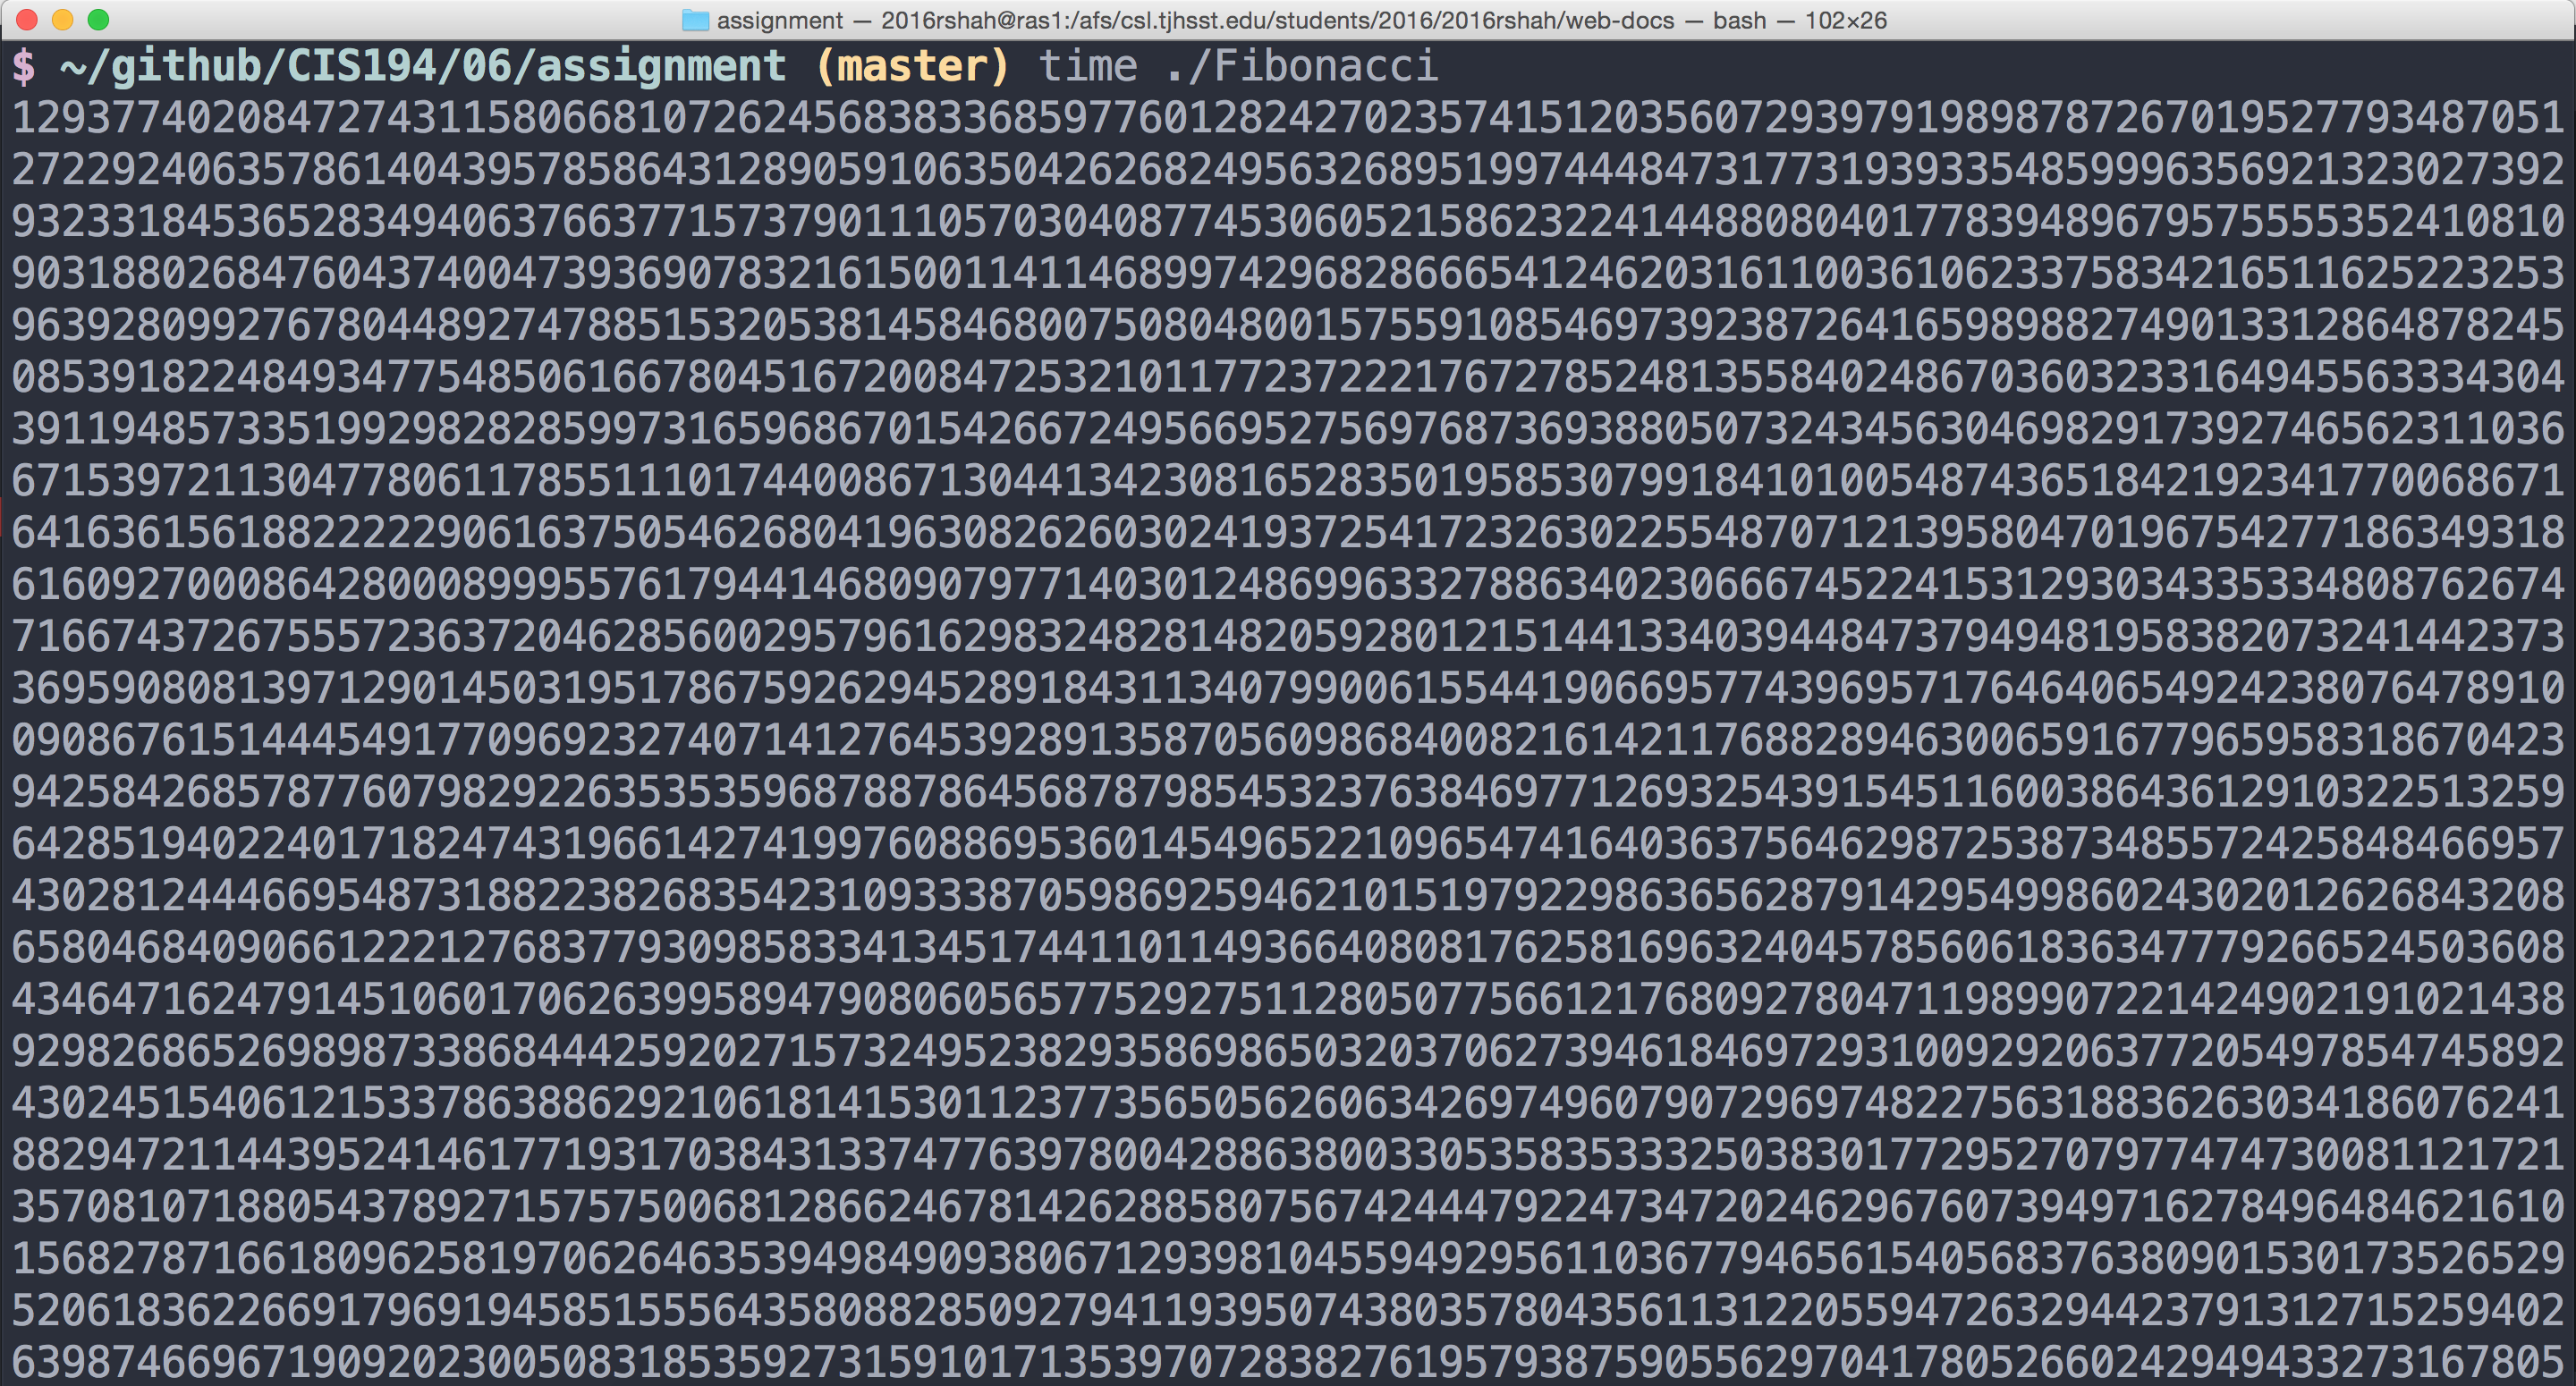
\includegraphics[width=6in]{Fibonacci_ss_1}

	\ldots\newline{}

	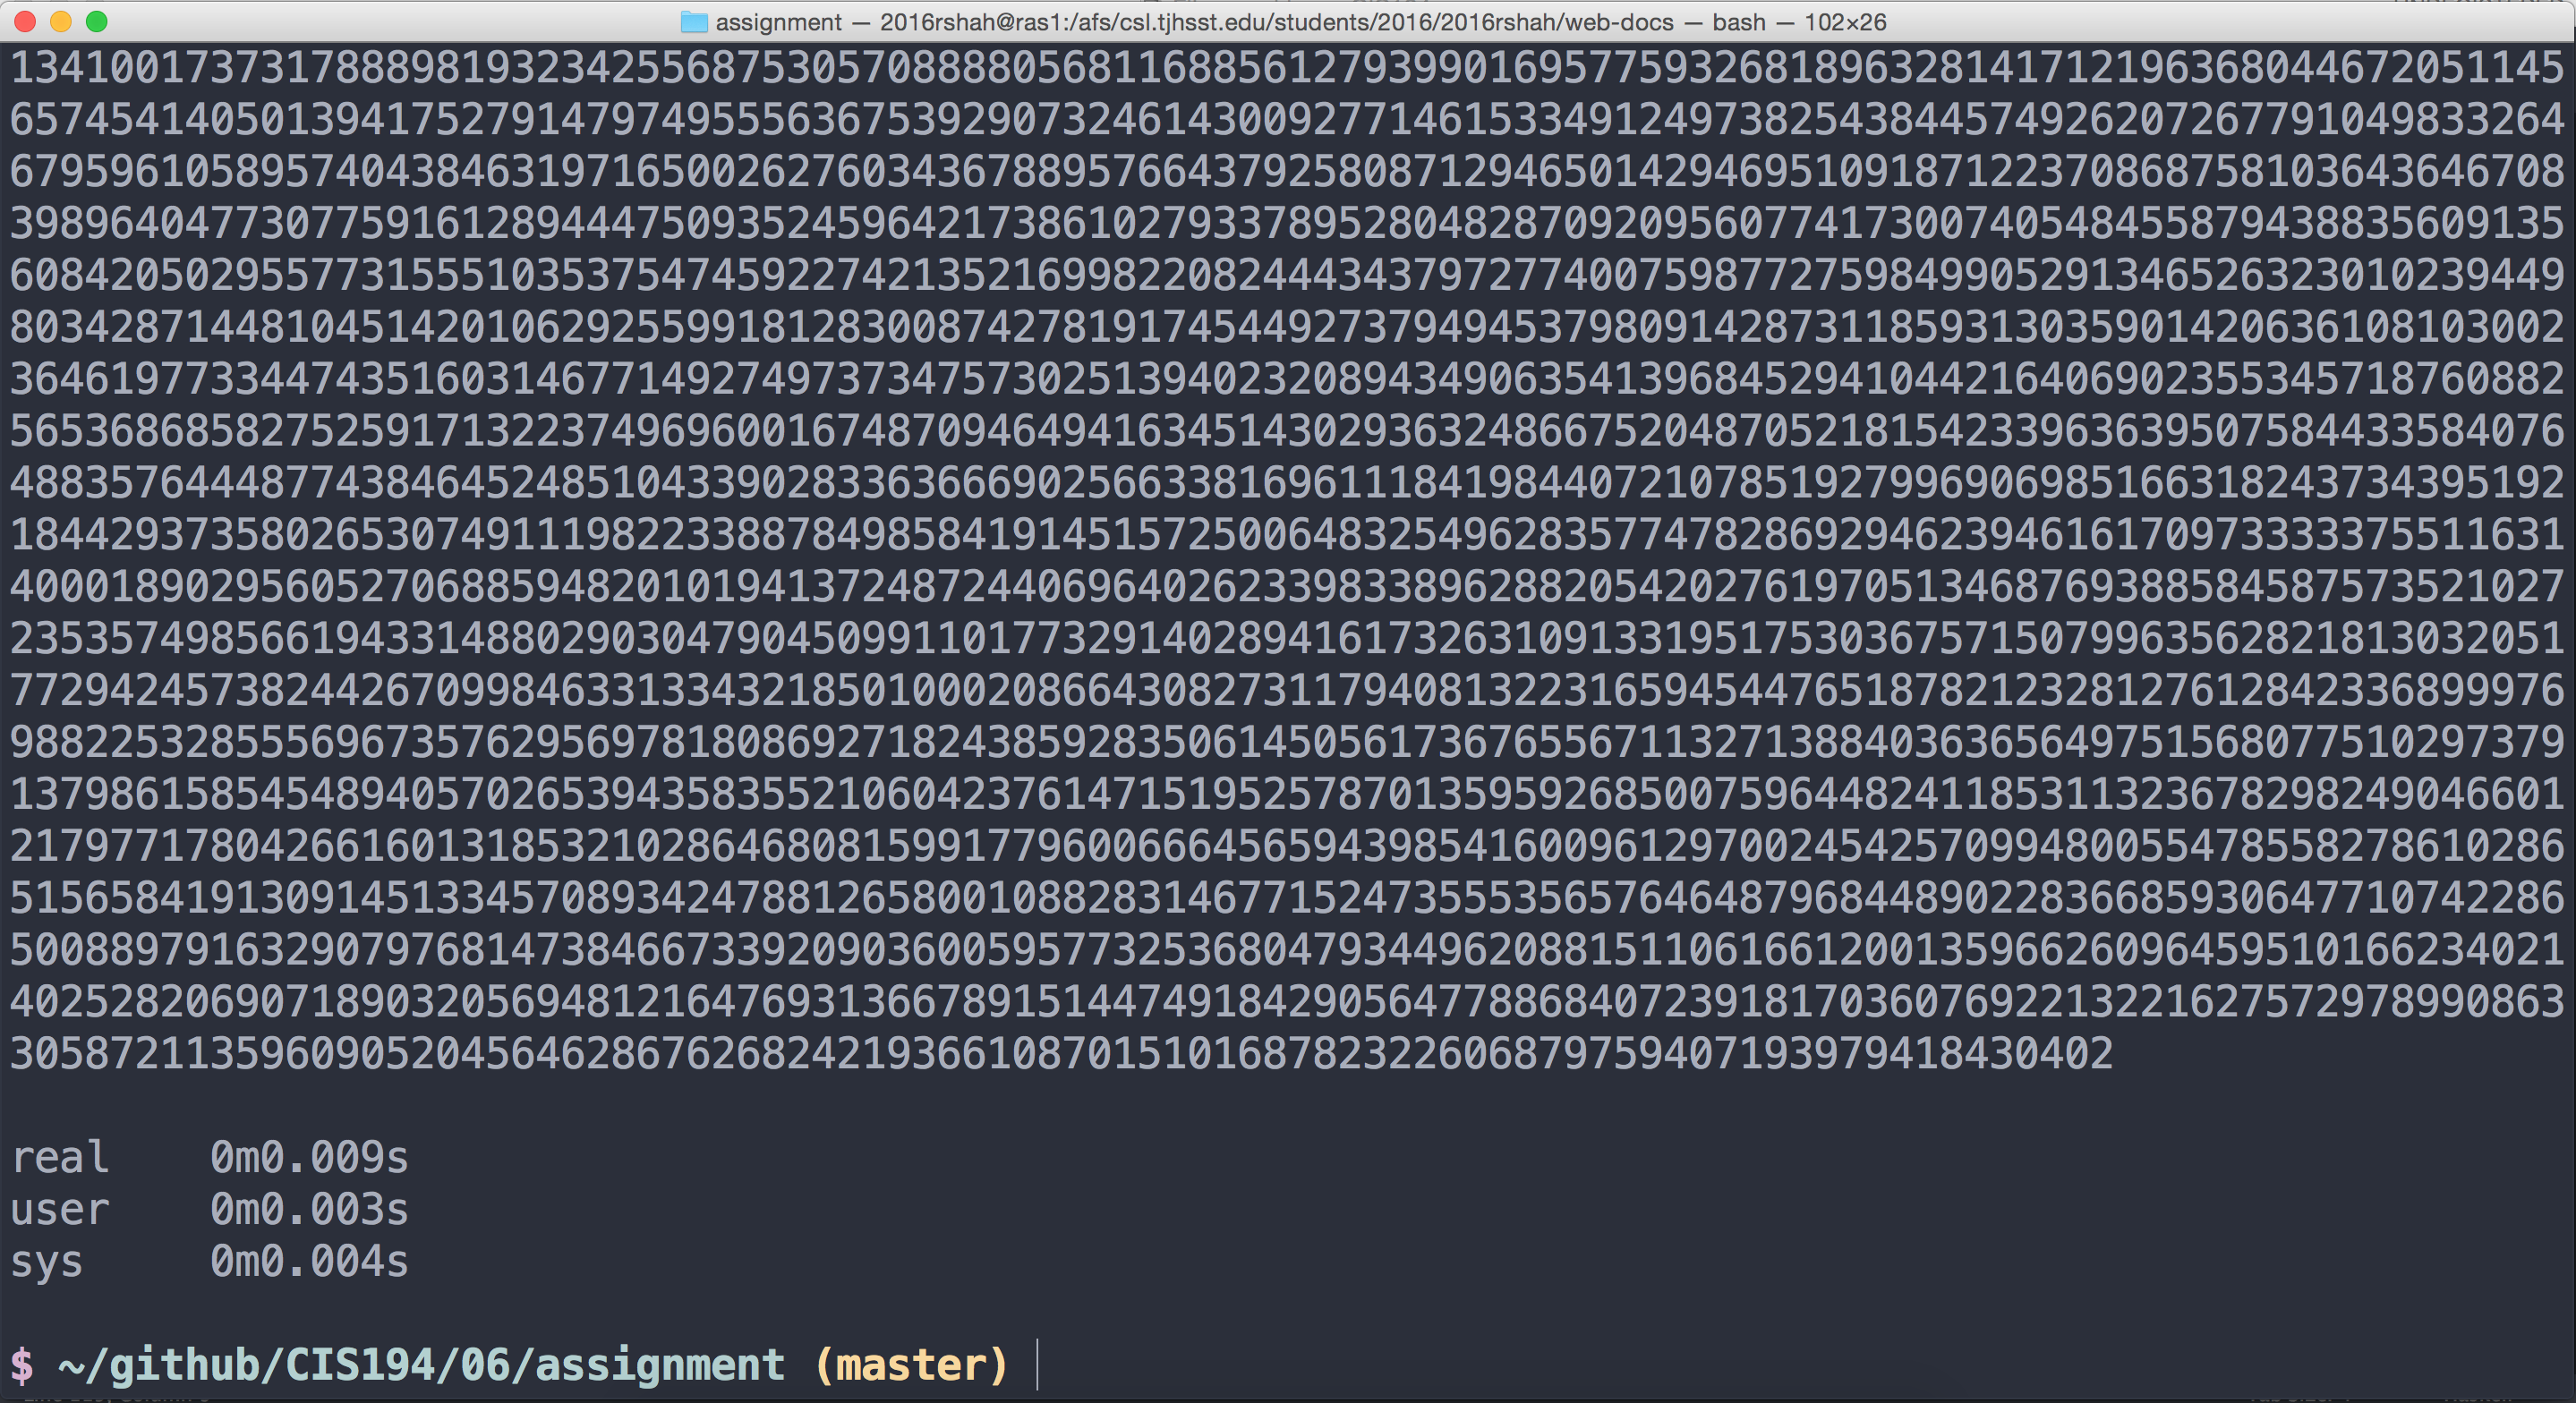
\includegraphics[width=6in]{Fibonacci_ss_2}

	That's right, the answer is a \texttt{8652} digit number, and was
	calculated in about \texttt{.009} seconds. If you want to see the
	answer, check out \href{http://www.rshah.org/blog/resources/Fibonacci_answer.txt}{this .txt file}.
\end{document}
